% Generated by Sphinx.
\def\sphinxdocclass{report}
\documentclass[letterpaper,10pt,english]{sphinxmanual}
\usepackage[utf8]{inputenc}
\DeclareUnicodeCharacter{00A0}{\nobreakspace}
\usepackage{cmap}
\usepackage[T1]{fontenc}
\usepackage{babel}
\usepackage{times}
\usepackage[Bjarne]{fncychap}
\usepackage{longtable}
\usepackage{sphinx}
\usepackage{multirow}


\title{Documentação Solar 2}
\date{August 14, 2014}
\release{2.0.0}
\author{Universidade Federal do Ceara, Instituto Universidade Virtual}
\newcommand{\sphinxlogo}{}
\renewcommand{\releasename}{Release}
\makeindex

\makeatletter
\def\PYG@reset{\let\PYG@it=\relax \let\PYG@bf=\relax%
    \let\PYG@ul=\relax \let\PYG@tc=\relax%
    \let\PYG@bc=\relax \let\PYG@ff=\relax}
\def\PYG@tok#1{\csname PYG@tok@#1\endcsname}
\def\PYG@toks#1+{\ifx\relax#1\empty\else%
    \PYG@tok{#1}\expandafter\PYG@toks\fi}
\def\PYG@do#1{\PYG@bc{\PYG@tc{\PYG@ul{%
    \PYG@it{\PYG@bf{\PYG@ff{#1}}}}}}}
\def\PYG#1#2{\PYG@reset\PYG@toks#1+\relax+\PYG@do{#2}}

\expandafter\def\csname PYG@tok@gd\endcsname{\def\PYG@tc##1{\textcolor[rgb]{0.63,0.00,0.00}{##1}}}
\expandafter\def\csname PYG@tok@gu\endcsname{\let\PYG@bf=\textbf\def\PYG@tc##1{\textcolor[rgb]{0.50,0.00,0.50}{##1}}}
\expandafter\def\csname PYG@tok@gt\endcsname{\def\PYG@tc##1{\textcolor[rgb]{0.00,0.27,0.87}{##1}}}
\expandafter\def\csname PYG@tok@gs\endcsname{\let\PYG@bf=\textbf}
\expandafter\def\csname PYG@tok@gr\endcsname{\def\PYG@tc##1{\textcolor[rgb]{1.00,0.00,0.00}{##1}}}
\expandafter\def\csname PYG@tok@cm\endcsname{\let\PYG@it=\textit\def\PYG@tc##1{\textcolor[rgb]{0.25,0.50,0.56}{##1}}}
\expandafter\def\csname PYG@tok@vg\endcsname{\def\PYG@tc##1{\textcolor[rgb]{0.73,0.38,0.84}{##1}}}
\expandafter\def\csname PYG@tok@m\endcsname{\def\PYG@tc##1{\textcolor[rgb]{0.13,0.50,0.31}{##1}}}
\expandafter\def\csname PYG@tok@mh\endcsname{\def\PYG@tc##1{\textcolor[rgb]{0.13,0.50,0.31}{##1}}}
\expandafter\def\csname PYG@tok@cs\endcsname{\def\PYG@tc##1{\textcolor[rgb]{0.25,0.50,0.56}{##1}}\def\PYG@bc##1{\setlength{\fboxsep}{0pt}\colorbox[rgb]{1.00,0.94,0.94}{\strut ##1}}}
\expandafter\def\csname PYG@tok@ge\endcsname{\let\PYG@it=\textit}
\expandafter\def\csname PYG@tok@vc\endcsname{\def\PYG@tc##1{\textcolor[rgb]{0.73,0.38,0.84}{##1}}}
\expandafter\def\csname PYG@tok@il\endcsname{\def\PYG@tc##1{\textcolor[rgb]{0.13,0.50,0.31}{##1}}}
\expandafter\def\csname PYG@tok@go\endcsname{\def\PYG@tc##1{\textcolor[rgb]{0.20,0.20,0.20}{##1}}}
\expandafter\def\csname PYG@tok@cp\endcsname{\def\PYG@tc##1{\textcolor[rgb]{0.00,0.44,0.13}{##1}}}
\expandafter\def\csname PYG@tok@gi\endcsname{\def\PYG@tc##1{\textcolor[rgb]{0.00,0.63,0.00}{##1}}}
\expandafter\def\csname PYG@tok@gh\endcsname{\let\PYG@bf=\textbf\def\PYG@tc##1{\textcolor[rgb]{0.00,0.00,0.50}{##1}}}
\expandafter\def\csname PYG@tok@ni\endcsname{\let\PYG@bf=\textbf\def\PYG@tc##1{\textcolor[rgb]{0.84,0.33,0.22}{##1}}}
\expandafter\def\csname PYG@tok@nl\endcsname{\let\PYG@bf=\textbf\def\PYG@tc##1{\textcolor[rgb]{0.00,0.13,0.44}{##1}}}
\expandafter\def\csname PYG@tok@nn\endcsname{\let\PYG@bf=\textbf\def\PYG@tc##1{\textcolor[rgb]{0.05,0.52,0.71}{##1}}}
\expandafter\def\csname PYG@tok@no\endcsname{\def\PYG@tc##1{\textcolor[rgb]{0.38,0.68,0.84}{##1}}}
\expandafter\def\csname PYG@tok@na\endcsname{\def\PYG@tc##1{\textcolor[rgb]{0.25,0.44,0.63}{##1}}}
\expandafter\def\csname PYG@tok@nb\endcsname{\def\PYG@tc##1{\textcolor[rgb]{0.00,0.44,0.13}{##1}}}
\expandafter\def\csname PYG@tok@nc\endcsname{\let\PYG@bf=\textbf\def\PYG@tc##1{\textcolor[rgb]{0.05,0.52,0.71}{##1}}}
\expandafter\def\csname PYG@tok@nd\endcsname{\let\PYG@bf=\textbf\def\PYG@tc##1{\textcolor[rgb]{0.33,0.33,0.33}{##1}}}
\expandafter\def\csname PYG@tok@ne\endcsname{\def\PYG@tc##1{\textcolor[rgb]{0.00,0.44,0.13}{##1}}}
\expandafter\def\csname PYG@tok@nf\endcsname{\def\PYG@tc##1{\textcolor[rgb]{0.02,0.16,0.49}{##1}}}
\expandafter\def\csname PYG@tok@si\endcsname{\let\PYG@it=\textit\def\PYG@tc##1{\textcolor[rgb]{0.44,0.63,0.82}{##1}}}
\expandafter\def\csname PYG@tok@s2\endcsname{\def\PYG@tc##1{\textcolor[rgb]{0.25,0.44,0.63}{##1}}}
\expandafter\def\csname PYG@tok@vi\endcsname{\def\PYG@tc##1{\textcolor[rgb]{0.73,0.38,0.84}{##1}}}
\expandafter\def\csname PYG@tok@nt\endcsname{\let\PYG@bf=\textbf\def\PYG@tc##1{\textcolor[rgb]{0.02,0.16,0.45}{##1}}}
\expandafter\def\csname PYG@tok@nv\endcsname{\def\PYG@tc##1{\textcolor[rgb]{0.73,0.38,0.84}{##1}}}
\expandafter\def\csname PYG@tok@s1\endcsname{\def\PYG@tc##1{\textcolor[rgb]{0.25,0.44,0.63}{##1}}}
\expandafter\def\csname PYG@tok@gp\endcsname{\let\PYG@bf=\textbf\def\PYG@tc##1{\textcolor[rgb]{0.78,0.36,0.04}{##1}}}
\expandafter\def\csname PYG@tok@sh\endcsname{\def\PYG@tc##1{\textcolor[rgb]{0.25,0.44,0.63}{##1}}}
\expandafter\def\csname PYG@tok@ow\endcsname{\let\PYG@bf=\textbf\def\PYG@tc##1{\textcolor[rgb]{0.00,0.44,0.13}{##1}}}
\expandafter\def\csname PYG@tok@sx\endcsname{\def\PYG@tc##1{\textcolor[rgb]{0.78,0.36,0.04}{##1}}}
\expandafter\def\csname PYG@tok@bp\endcsname{\def\PYG@tc##1{\textcolor[rgb]{0.00,0.44,0.13}{##1}}}
\expandafter\def\csname PYG@tok@c1\endcsname{\let\PYG@it=\textit\def\PYG@tc##1{\textcolor[rgb]{0.25,0.50,0.56}{##1}}}
\expandafter\def\csname PYG@tok@kc\endcsname{\let\PYG@bf=\textbf\def\PYG@tc##1{\textcolor[rgb]{0.00,0.44,0.13}{##1}}}
\expandafter\def\csname PYG@tok@c\endcsname{\let\PYG@it=\textit\def\PYG@tc##1{\textcolor[rgb]{0.25,0.50,0.56}{##1}}}
\expandafter\def\csname PYG@tok@mf\endcsname{\def\PYG@tc##1{\textcolor[rgb]{0.13,0.50,0.31}{##1}}}
\expandafter\def\csname PYG@tok@err\endcsname{\def\PYG@bc##1{\setlength{\fboxsep}{0pt}\fcolorbox[rgb]{1.00,0.00,0.00}{1,1,1}{\strut ##1}}}
\expandafter\def\csname PYG@tok@kd\endcsname{\let\PYG@bf=\textbf\def\PYG@tc##1{\textcolor[rgb]{0.00,0.44,0.13}{##1}}}
\expandafter\def\csname PYG@tok@ss\endcsname{\def\PYG@tc##1{\textcolor[rgb]{0.32,0.47,0.09}{##1}}}
\expandafter\def\csname PYG@tok@sr\endcsname{\def\PYG@tc##1{\textcolor[rgb]{0.14,0.33,0.53}{##1}}}
\expandafter\def\csname PYG@tok@mo\endcsname{\def\PYG@tc##1{\textcolor[rgb]{0.13,0.50,0.31}{##1}}}
\expandafter\def\csname PYG@tok@mi\endcsname{\def\PYG@tc##1{\textcolor[rgb]{0.13,0.50,0.31}{##1}}}
\expandafter\def\csname PYG@tok@kn\endcsname{\let\PYG@bf=\textbf\def\PYG@tc##1{\textcolor[rgb]{0.00,0.44,0.13}{##1}}}
\expandafter\def\csname PYG@tok@o\endcsname{\def\PYG@tc##1{\textcolor[rgb]{0.40,0.40,0.40}{##1}}}
\expandafter\def\csname PYG@tok@kr\endcsname{\let\PYG@bf=\textbf\def\PYG@tc##1{\textcolor[rgb]{0.00,0.44,0.13}{##1}}}
\expandafter\def\csname PYG@tok@s\endcsname{\def\PYG@tc##1{\textcolor[rgb]{0.25,0.44,0.63}{##1}}}
\expandafter\def\csname PYG@tok@kp\endcsname{\def\PYG@tc##1{\textcolor[rgb]{0.00,0.44,0.13}{##1}}}
\expandafter\def\csname PYG@tok@w\endcsname{\def\PYG@tc##1{\textcolor[rgb]{0.73,0.73,0.73}{##1}}}
\expandafter\def\csname PYG@tok@kt\endcsname{\def\PYG@tc##1{\textcolor[rgb]{0.56,0.13,0.00}{##1}}}
\expandafter\def\csname PYG@tok@sc\endcsname{\def\PYG@tc##1{\textcolor[rgb]{0.25,0.44,0.63}{##1}}}
\expandafter\def\csname PYG@tok@sb\endcsname{\def\PYG@tc##1{\textcolor[rgb]{0.25,0.44,0.63}{##1}}}
\expandafter\def\csname PYG@tok@k\endcsname{\let\PYG@bf=\textbf\def\PYG@tc##1{\textcolor[rgb]{0.00,0.44,0.13}{##1}}}
\expandafter\def\csname PYG@tok@se\endcsname{\let\PYG@bf=\textbf\def\PYG@tc##1{\textcolor[rgb]{0.25,0.44,0.63}{##1}}}
\expandafter\def\csname PYG@tok@sd\endcsname{\let\PYG@it=\textit\def\PYG@tc##1{\textcolor[rgb]{0.25,0.44,0.63}{##1}}}

\def\PYGZbs{\char`\\}
\def\PYGZus{\char`\_}
\def\PYGZob{\char`\{}
\def\PYGZcb{\char`\}}
\def\PYGZca{\char`\^}
\def\PYGZam{\char`\&}
\def\PYGZlt{\char`\<}
\def\PYGZgt{\char`\>}
\def\PYGZsh{\char`\#}
\def\PYGZpc{\char`\%}
\def\PYGZdl{\char`\$}
\def\PYGZhy{\char`\-}
\def\PYGZsq{\char`\'}
\def\PYGZdq{\char`\"}
\def\PYGZti{\char`\~}
% for compatibility with earlier versions
\def\PYGZat{@}
\def\PYGZlb{[}
\def\PYGZrb{]}
\makeatother

\begin{document}

\maketitle
\tableofcontents
\phantomsection\label{index::doc}


Diante das dimensões dos recursos e das ferramentas disponibilizadas pela versão 2 do \textbf{Solar}, iniciaremos através desse tutorial e de seu conteúdo, que integra: imagens, textos e vídeos, o compartilhamento de informações e a divulgação de atualizações do ambiente \textbf{Solar 2}.

Este manual possui como um dos seus principais focos o detalhamento das funcionalidades disponíveis para cada perfil de usuário, seja elas: Fóruns, Chats, Webconferências, administração de usuários, etc. Além disso, temos ainda em suas páginas uma lista de {\hyperref[faq::doc]{\emph{Perguntas Frequentes (FAQ)}}} , que será atualizada progressivamente.

Sendo o \textbf{Solar 2} um AVA (Ambiente Virtual de Aprendizagem), gradativamente irá incorporar outras redes sociais, ferramentas de edição e simuladores; servindo dessa forma como elemento convergente de aplicações voltadas e/ou desenvolvidas para aprendizagem. Com essa perspectiva e necessária a existência de um local que dinamize a compreensão e a assimilação rápida e eficaz de todos os componentes do sistema.
Nosso desejo é que esse espaço sirva para esclarecimentos, tira-dúvidas e suporte para capacitações e/ou treinamentos.

\emph{Instituto UFC Virtual, Universidade Federal do Ceará}


\chapter{Ambiente}
\label{index:projeto-solar-2-0}\label{index:ambiente}

\section{Acesso ao Sistema}
\label{access:access}\label{access:acesso-ao-sistema}\label{access::doc}
Neste tutorial, apresentamos as opções:
\begin{itemize}
\item {} 
{\hyperref[access:login]{Login}}

\item {} 
{\hyperref[access:cadastro-de-usuario]{Cadastro de usuário}}

\item {} 
{\hyperref[access:recuperacao-de-senha]{Recuperação de senha}}

\item {} 
{\hyperref[access:saindo-do-sistema]{Saindo do sistema}}

\end{itemize}


\subsection{Login}
\label{access:login}\label{access:id1}
Caso o usuário já possua uma Login e senha cadastrada, basta inserir estes dados e clicar em \textbf{Acessar}. A próxima página apresentada será a Home do sistema.
\begin{figure}[htbp]
\centering
\capstart

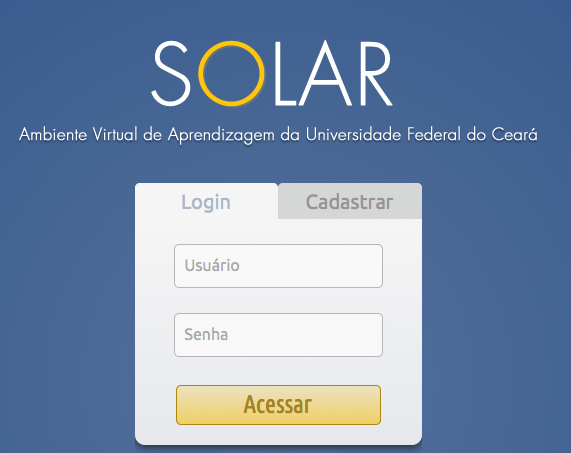
\includegraphics{login-01.png}
\caption{Tela inicial do Ambiente Solar}\end{figure}


\subsection{Cadastro de usuário}
\label{access:cadastro}\label{access:cadastro-de-usuario}
Para se cadastrar basta clicar em \textbf{Cadastrar}. Na tela seguinte será solicitado o e-mail e o CPF do usuário.
\begin{enumerate}
\item {} 
Inserir um CPF válido

\end{enumerate}

{\hfill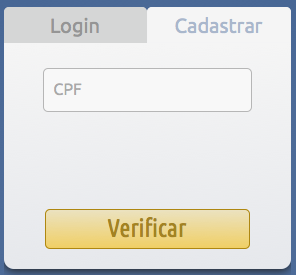
\includegraphics{register-01.png}\hfill}
\begin{enumerate}
\setcounter{enumi}{1}
\item {} 
Inserir dados pessoais

\end{enumerate}

{\hfill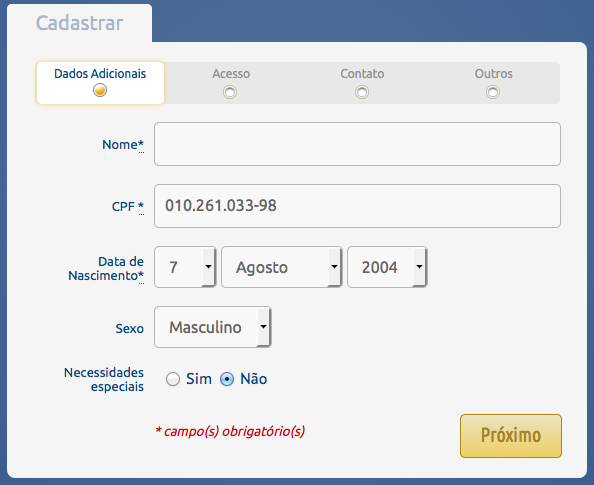
\includegraphics{register-02.png}\hfill}
\begin{enumerate}
\setcounter{enumi}{2}
\item {} 
Inserir dados de acesso

\end{enumerate}

{\hfill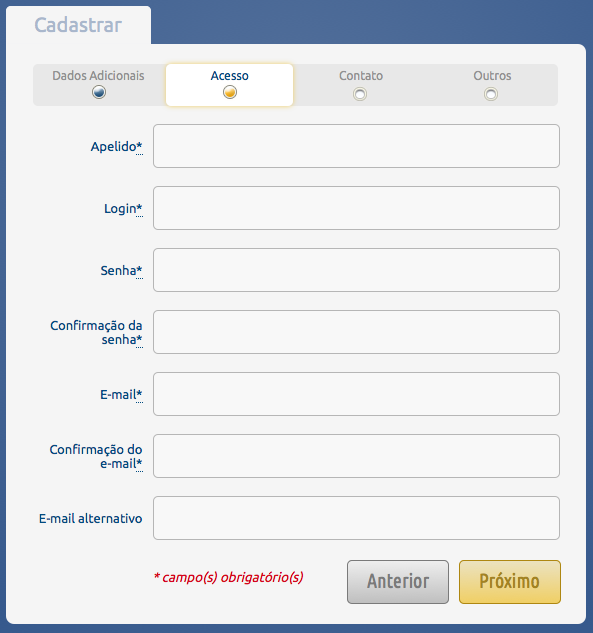
\includegraphics{register-03.png}\hfill}
\begin{enumerate}
\setcounter{enumi}{3}
\item {} 
Inserir dados de contato

\end{enumerate}

{\hfill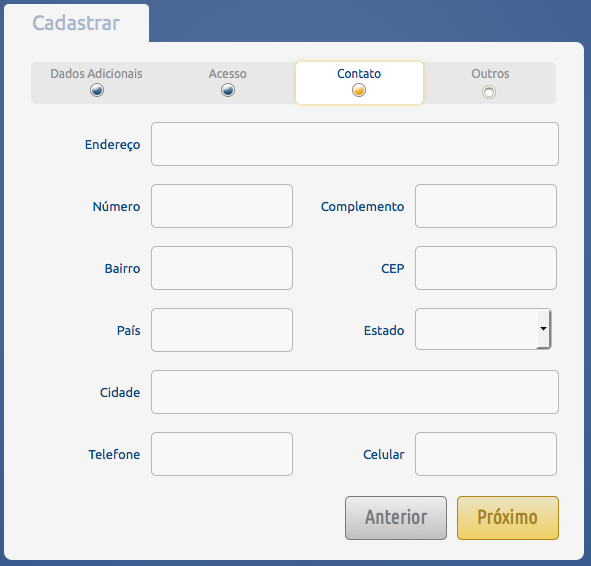
\includegraphics{register-04.png}\hfill}
\begin{enumerate}
\setcounter{enumi}{4}
\item {} 
Informar a instituição na qual você pertence

\end{enumerate}

{\hfill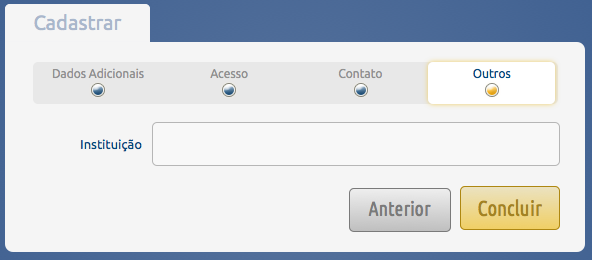
\includegraphics{register-05.png}\hfill}

Depois de concluído o cadastro o usuário já pode entrar no sistema normalmente.


\subsection{Recuperação de senha}
\label{access:recuperacao-de-senha}\label{access:recuperar-senha}
Caso já tenha um usuário, mas perdeu a senha, basta clicar em \textbf{Esqueceu a sua senha?} na tela de Login. Na próxima tela será solicitado o e-mail cadastrado.

{\hfill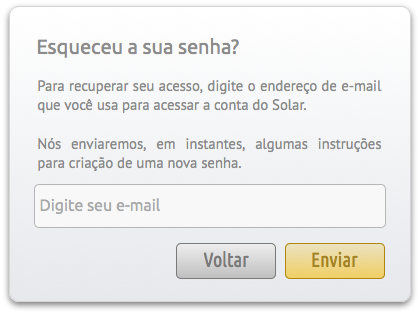
\includegraphics{password-01.png}\hfill}

Será enviada uma mensagem de confirmação para o endereço de e-mail informado.

{\hfill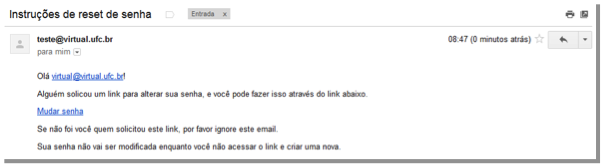
\includegraphics{password-02.png}\hfill}

Após clicar no link para mudar a senha, a tela abaixo será apresentada solicitando a alteração da senha.

{\hfill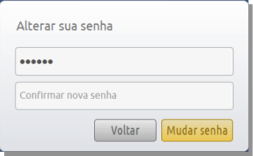
\includegraphics{password-03.png}\hfill}


\subsection{Saindo do sistema}
\label{access:saindo-do-sistema}\label{access:sair-sistema}
Para sair do sistema basta clicar em \textbf{Sair}, na barra superior.

{\hfill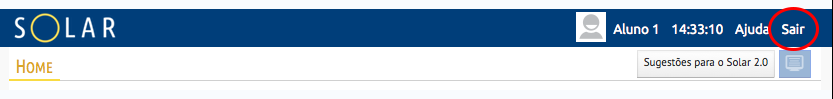
\includegraphics{logout-01.png}\hfill}

Após sair do sistema, será apresentada a mensagem \textbf{Logout efetuado com sucesso} na página de login.

{\hfill
\includegraphics{logout-02.png}\hfill}


\section{Matrícula}
\label{enrollment:matricula}\label{enrollment:enrollment}\label{enrollment::doc}
Neste tutorial apresentamos o módulo de Matricula e as seguintes funcionalidades:
\begin{itemize}
\item {} 
{\hyperref[enrollment:informacoes-gerais]{Informações gerais}}

\item {} 
{\hyperref[enrollment:acesso-a-matricula]{Acesso à matrícula}}

\item {} 
{\hyperref[enrollment:solicitar-matricula-em-uma-oferta]{Solicitar matrícula em uma oferta}}

\item {} 
{\hyperref[enrollment:cancelar-matricula-em-uma-unidade-curricular]{Cancelar matrícula em uma Unidade Curricular}}

\item {} 
{\hyperref[enrollment:gerenciar-matricula-de-usuarios]{Gerenciar matrícula de usuários}}
\begin{itemize}
\item {} 
{\hyperref[enrollment:verificando-status-dos-matriculados]{Verificando status dos matriculados}}

\item {} 
{\hyperref[enrollment:matriculando-aluno-s]{Matriculando aluno(s)}}

\end{itemize}

\end{itemize}


\subsection{Informações gerais}
\label{enrollment:informacoes-gerais}\label{enrollment:enrollment-info}
Após efetuar o devido Login no Solar 2.0, nos deparamos com o Home, página inicial do AVA.
\begin{figure}[htbp]
\centering
\capstart

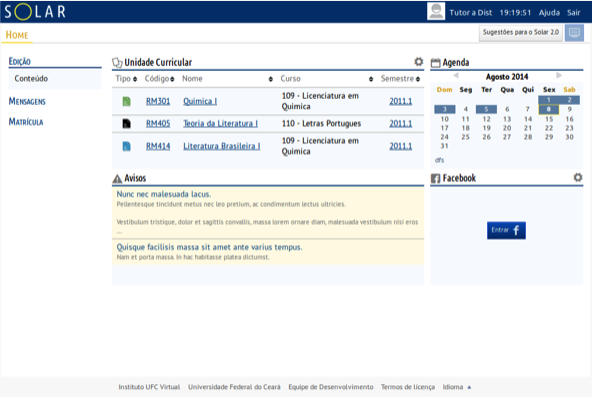
\includegraphics{enrollment-info.png}
\caption{Tela inicial após logar no sistema}\end{figure}
\begin{itemize}
\item {} 
Ao solicitar matrícula, o usuário estará solicitando que um perfil do tipo Aluno seja associado a ele para determinada disciplina.

\item {} 
Um perfil está associado a um conjunto de permissões que o usuário tem para realizar atividades no Solar 2.0.

\item {} 
Ao realizar a matrícula, o usuário deve aguardar o aceite dessa para que possa estar devidamente matriculado na disciplina desejada.

\item {} 
O Aceite de Matrícula é necessário para que um aluno possa cursar uma disciplina no Solar 2.0, exceto para as disciplinas dos cursos oferecidos pela UAB, pois a matricula destes é realizada pelo Módulo Acadêmico.

\end{itemize}


\subsection{Acesso à matrícula}
\label{enrollment:acesso-a-matricula}\label{enrollment:enrollment-access}
Ao acessar a tela de matrícula, o usuário se depara com quatro áreas. A \emph{primeira} é a área de Busca, na qual o usuário pode buscar pelo nome da disciplina, primeiro campo de busca, ou por seu tipo, segundo campo de busca.

Para realizar uma busca, o usuário deve preencher ao menos um dos dois campos e clicar no botão de \textbf{lupa} para realizar a busca
\begin{figure}[htbp]
\centering

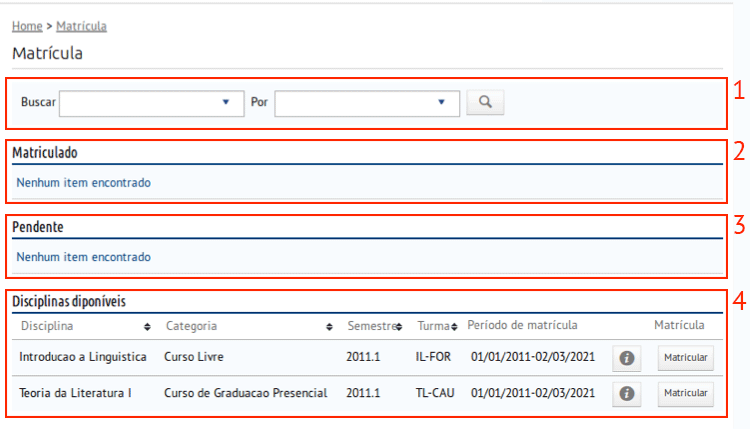
\includegraphics{enrollment-search.png}
\end{figure}

A \emph{segunda} área é uma lista de todas as disciplinas nas quais o usuário já está matriculado. Sendo que este pode, ou não, cancelar sua matrícula.

A \emph{terceira} área é uma lista com todas as matrículas pendentes realizadas pelo usuário. Ou seja, todos os pedidos de matrícula que ainda não foram aceitos.

A \emph{quarta} e última área é uma lista com todas as ofertas correntes (ou seja, cujo período de matrícula ainda está vigente) de disciplinas disponíveis para matrícula no sistema. O botão de informações abrirá a janela abaixo, que contém todas as informações disponíveis da oferta como detalhes da disciplina, período de vigência, período de matrícula e os responsáveis (professores, tutores etc) pela disciplina.
\begin{figure}[htbp]
\centering
\capstart

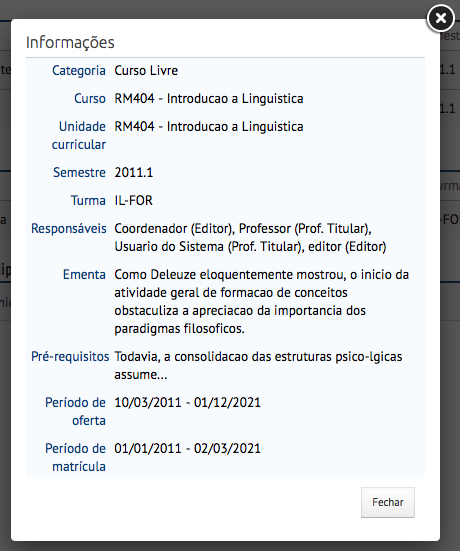
\includegraphics{enrollment-lightbox.png}
\caption{Lightbox de informações de uma oferta}\end{figure}

\begin{notice}{note}{Note:}
Ressaltamos que Disciplinas, no contexto do Solar 2.0, possuem os tipos:
\begin{itemize}
\item {} 
Curso de extensão;

\item {} 
Curso de Graduação a distância;

\item {} 
Curso de Graduação presencial;

\item {} 
Curso de Pós-graduação a distância;

\item {} 
Curso de Pós-graduação presencial;

\item {} 
Curso Livre.

\end{itemize}
\end{notice}


\subsection{Solicitar matrícula em uma oferta}
\label{enrollment:solicitar-matricula-em-uma-oferta}\label{enrollment:enrollment-request}
Para solicitar sua matrícula em alguma oferta de disciplina disponível, basta clicar em \textbf{Matricular}.
\begin{figure}[htbp]
\centering

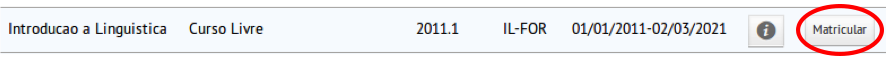
\includegraphics{enrollment-request.png}
\end{figure}

Ao clicar no botão informado, a seguinte mensagem de sucesso aparecerá.

{\hfill
\includegraphics{enrollment-request-success.png}\hfill}


\subsection{Cancelar matrícula em uma Unidade Curricular}
\label{enrollment:cancelar-matricula-em-uma-unidade-curricular}\label{enrollment:enrollment-cancel}
Para cancelar a matricula de Unidade Curricular, basta clicar no botão \textbf{Cancelar pedido}.

{\hfill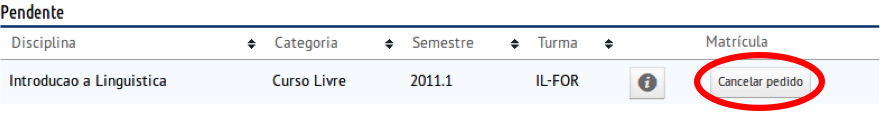
\includegraphics{enrollment-cancel-01.png}\hfill}

Será enviada uma mensagem de confirmação em seguida.

{\hfill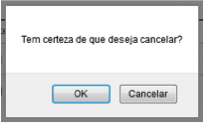
\includegraphics{enrollment-cancel-02.png}\hfill}


\subsection{Gerenciar matrícula de usuários}
\label{enrollment:enrollment-manage}\label{enrollment:gerenciar-matricula-de-usuarios}
\begin{notice}{attention}{Attention:}
Esta funcionalidade está disponível para o seguinte perfil: \textbf{Editor}
\end{notice}

Após efetuar o devido Login no Solar 2.0, na página inicial (\emph{Home}), o link de acesso à \emph{Gerenciar Matrículas} está localizado no menu de navegação à esquerda.

{\hfill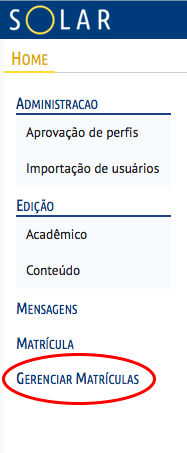
\includegraphics{enrollment-manage-01.png}\hfill}


\subsubsection{Verificando status dos matriculados}
\label{enrollment:verificando-status-dos-matriculados}
Nesta página é listado o estado de matrícula de todos os alunos do sistema.

{\hfill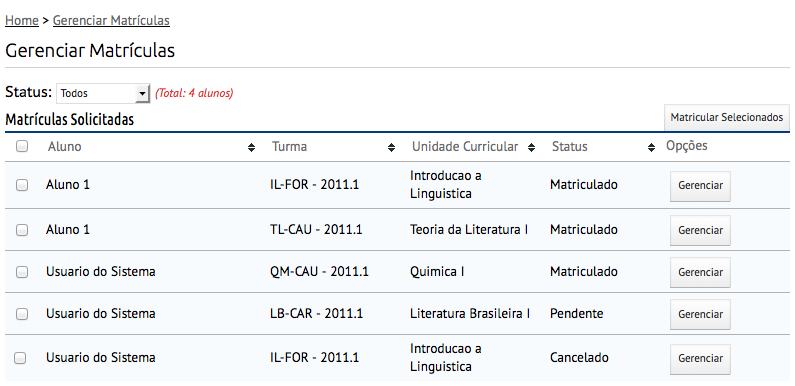
\includegraphics{enrollment-manage-02.png}\hfill}

Caso deseje filtrar esta lista, basta utilizar a lista de opções de \textbf{status}, que a lista será filtrada automaticamente.

{\hfill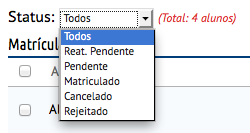
\includegraphics{enrollment-manage-03.png}\hfill}


\subsubsection{Matriculando aluno(s)}
\label{enrollment:matriculando-aluno-s}
\begin{notice}{note}{Note:}
Caso seja acionado o botão \textbf{Gerenciar} ou o botão \textbf{Matricular Selecionados} sem que nenhum aluno tenha sido selecionado, a mensagem \textbf{Nenhum registro selecionado} será exibida.
\end{notice}

Para matricular um aluno, basta pressionar o botão \textbf{Gerenciar} . Serão exibidas as opções do aluno conforme apresentado abaixo.

{\hfill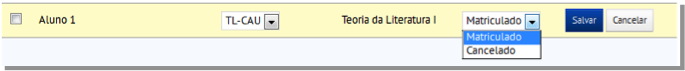
\includegraphics{enrollment-manage-04.png}\hfill}
\begin{enumerate}
\item {} 
No item 1 escolha a turma

\item {} 
No item 2 escolha se deseja o status de: \emph{MATRICULADO} ou \emph{CANCELADO}.

\item {} 
Após escolhidas às opções clique em \textbf{Salvar}.

\end{enumerate}

Para matricular vários alunos, basta marcar a caixa de seleção ao lado do nome de cada aluno e o botão \textbf{Matricular Selecionados} . Não serão exibidas as opções do aluno.

{\hfill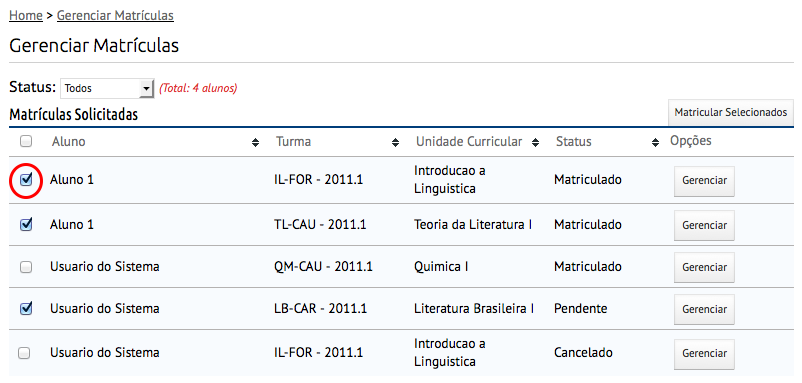
\includegraphics{enrollment-manage-05.png}\hfill}


\section{Mensagens}
\label{messages:mensagens}\label{messages:message}\label{messages::doc}
O link de acesso à página de \textbf{Mensagens} encontra-se no menu de navegação, localizado na lateral esquerda da página. Este tutorial apresentará as seguintes funcionalidades:
\begin{itemize}
\item {} 
{\hyperref[messages:mensagens-recebidas]{Mensagens recebidas}}

\item {} 
{\hyperref[messages:mensagens-enviadas]{Mensagens enviadas}}

\item {} 
{\hyperref[messages:mensagens-excluidas]{Mensagens excluídas}}

\item {} 
{\hyperref[messages:criar-uma-nova-mensagem]{Criar uma nova mensagem}}

\end{itemize}


\subsection{Mensagens recebidas}
\label{messages:mensagens-recebidas}
Nesta página constam todas as mensagens recebidas pelo usuário.
\begin{figure}[htbp]
\centering
\capstart

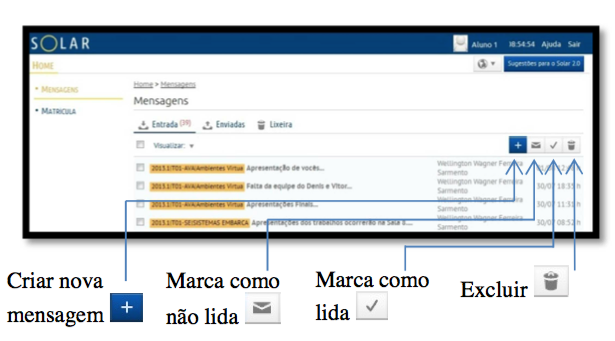
\includegraphics{messages-inbox.png}
\caption{Tela inicial de Mensagens}\end{figure}

No link \textbf{Visualizar} podemos filtrar as mensagens entre três tipo: Todas, Lidas, Não Lidas.
\begin{figure}[htbp]
\centering
\capstart

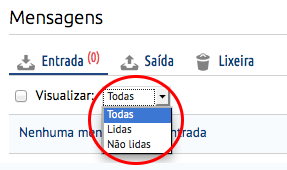
\includegraphics{messages-filter.png}
\caption{Filtrar mensagens por status}\end{figure}


\subsection{Mensagens enviadas}
\label{messages:mensagens-enviadas}
Para verificar as mensagens enviadas, basta clicar em \textbf{Enviadas} na barra de mensagens.


\subsection{Mensagens excluídas}
\label{messages:mensagens-excluidas}
Para verificar as uma mensagens excluidas basta clicar em \textbf{Lixeira} na barra de mensagens. Caso seja necessário recuperar uma mensagem, selecione a mensagem e clique no botão 
\includegraphics{messages-btn-restore.png} (\emph{Restaurar Mensagem}).


\subsection{Criar uma nova mensagem}
\label{messages:criar-uma-nova-mensagem}
Para criar uma nova mensagem clique no botão 
\includegraphics{messages-btn-new.png} (\emph{Nova Mensagem}), onde será apresentado um editor para você compor seu texto.
\begin{figure}[htbp]
\centering
\capstart

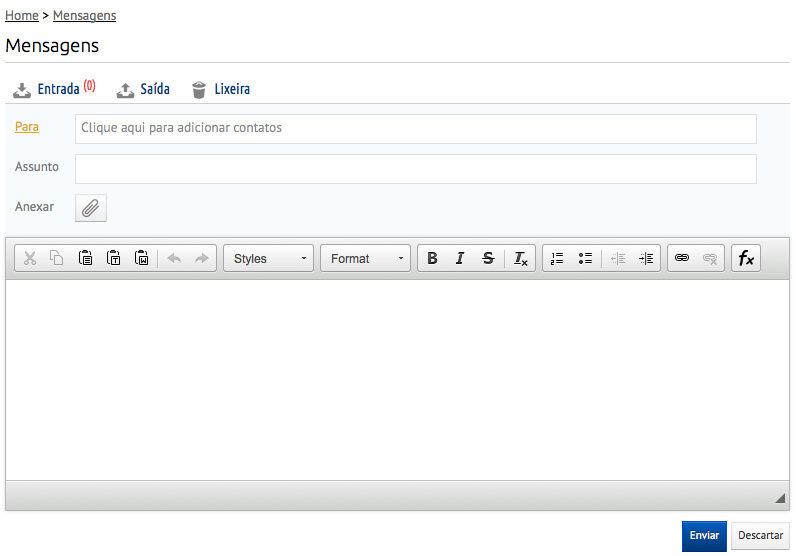
\includegraphics{messages-compose.png}
\caption{Composição de mensagem}\end{figure}

Ao clicar no campo \textbf{Para} lhe será apresentado uma janela para selecionar a quais contatos deseja enviar a mensagem, onde primeiramente você de qual Unidade Curricular eles pertencem. Para escolher para quem se deseja enviar a mensagem, basta clicar no nome do usuário. O nome escolhido irá para caixa inferior.
\begin{figure}[htbp]
\centering
\capstart

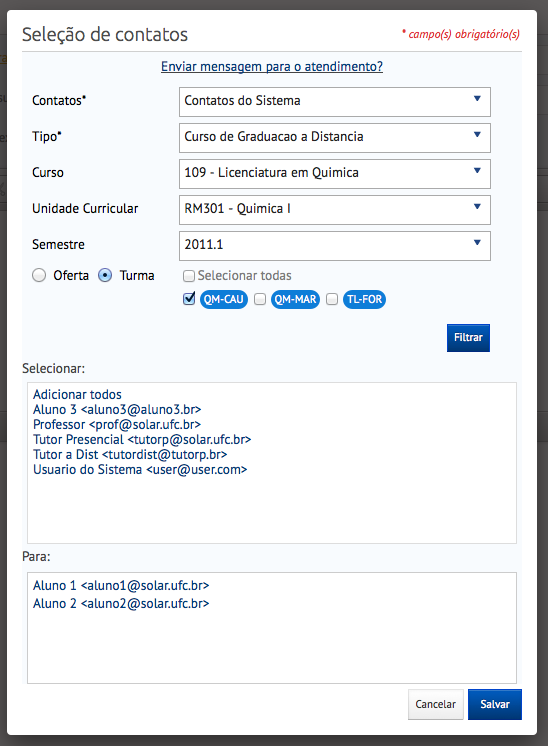
\includegraphics{messages-compose-lightbox.png}
\caption{Lightbox de seleção de contatos}\end{figure}

Para enviar a mensagem basta clicar no botão \textbf{Enviar}, da mesma forma podemos cancelar o processo clicando no botão \textbf{Descartar}.


\section{Perguntas Frequentes (FAQ)}
\label{faq:perguntas-frequentes-faq}\label{faq::doc}

\subsection{O que fazer se esqueci minha senha?}
\label{faq:o-que-fazer-se-esqueci-minha-senha}

\subsubsection{Sou aluno ou professor dos cursos da UAB}
\label{faq:sou-aluno-ou-professor-dos-cursos-da-uab}
Dirija-se à \href{https://www.moduloacademico.ufc.br/moduloacademico/guest/recuperarSenhaForm.do}{recuperação de senha do Módulo Acadêmico} a fim de recuperar sua senha. Após recuperar e alterar sua senha, retorne ao Solar 2.0 e utilize o mesmo login e senha do Módulo Acadêmico. Se você não consegue recuperar sua senha no Módulo Acadêmico, favor dirigir-se à secretaria de seu curso.


\subsubsection{Não sou aluno nem professor dos cursos da UAB, mas sou tutor ou coordenador}
\label{faq:nao-sou-aluno-nem-professor-dos-cursos-da-uab-mas-sou-tutor-ou-coordenador}\begin{itemize}
\item {} 
Possuo acesso ao Módulo Acadêmico

Dirija-se à \href{https://www.moduloacademico.ufc.br/moduloacademico/guest/recuperarSenhaForm.do}{recuperação de senha do Módulo Acadêmico} a fim de recuperar sua senha.

Após recuperar e alterar sua senha, retorne ao Solar 2.0 e utilize o mesmo login e senha do Módulo Acadêmico.

\item {} 
Não possuo acesso ao Módulo Acadêmico

Na tela de login do \href{http://www.solar.virtual.ufc.br}{Solar 2.0}, clique em \textbf{Esqueceu a sua senha?}, informe o email cadastrado e clique em `Enviar'.
\begin{itemize}
\item {} 
Recebi a seguinte mensagem me direcionando ao Módulo Acadêmico: \emph{`Para recuperar seus dados de acesso, vá ao endereço: https://www.moduloacademico.ufc.br/moduloacademico'}

Entre em contato com o \href{mailto:atendimento@virtual.ufc.br}{atendimento@virtual.ufc.br} relatando a situação e aguarde um email para recuperação de senha.

\item {} 
Recebi a seguinte mensagem: \emph{`Você receberá um email com instruções sobre como resetar sua senha em alguns minutos'}

Aguarde o email para recuperação de senha.

\item {} 
Recebi a mensagem: \emph{`E-mail não encontrado'}

Entre em contato com o \href{mailto:atendimento@virtual.ufc.br}{atendimento@virtual.ufc.br} relatando a situação, informe o cpf e aguarde um email para recuperação de senha.

\end{itemize}

\end{itemize}


\subsubsection{Não estou vinculado aos cursos da UAB}
\label{faq:nao-estou-vinculado-aos-cursos-da-uab}
Na tela de login do \href{http://www.solar.virtual.ufc.br}{Solar 2.0}, clique em \textbf{Esqueceu a sua senha?}, informe o email cadastrado e clique em `Enviar'. Aguarde o email para recuperação de senha.


\subsection{O que fazer para acessar o Solar 2.0 pela primeira vez?}
\label{faq:o-que-fazer-para-acessar-o-solar-2-0-pela-primeira-vez}

\subsubsection{Sou aluno ou professor dos cursos da UAB}
\label{faq:id1}
Utilize o mesmo login e senha do Módulo Acadêmico.
\begin{itemize}
\item {} 
Recebi uma mensagem de \emph{`Usuário ou senha inválidos'}

Acesse a aba \textbf{Cadastrar} e clique em \textbf{Verificar}.
\begin{itemize}
\item {} 
Recebi uma mensagem \emph{`Seus dados de acesso foram importados do Módulo Acadêmico. Para alterar ou recuperar seus dados de acesso, vá ao endereço: https://www.moduloacademico.ufc.br/moduloacademico'}

\end{itemize}

Seus dados foram importados do Módulo Acadêmico. Utilize o mesmo login e senha do Módulo Acadêmico para efetuar o login no sistema.

\end{itemize}


\subsubsection{Não sou aluno nem professor dos cursos da UAB, mas sou tutor ou coordenador}
\label{faq:id2}
Tente efetuar o login com os dados prévios do Solar 1.2
\begin{itemize}
\item {} 
Recebi uma mensagem de \emph{`Usuário ou senha inválidos'}

Acesse a aba \textbf{Cadastrar} e clique em \textbf{Verificar}.
\begin{itemize}
\item {} 
Recebi uma mensagem \emph{`Seus dados de acesso foram importados do Módulo Acadêmico. Para alterar ou recuperar seus dados de acesso, vá ao endereço: https://www.moduloacademico.ufc.br/moduloacademico'}
\begin{itemize}
\item {} 
Não possuo acesso ao Módulo Acadêmico

Entre em contato com o \href{mailto:atendimento@virtual.ufc.br}{atendimento@virtual.ufc.br} relatando a situação e aguarde um email para recuperação de senha.
\begin{itemize}
\item {} 
O atendimento me retornou informando que meus dados não podem ser alterados?

Acesse a \href{https://www.moduloacademico.ufc.br/moduloacademico/guest/recuperarSenhaForm.do}{recuperação de senha do Módulo Acadêmico}. Coloque, no login, o número do seu CPF e, na senha, seu primeiro nome em letras maiúsculas. Após conseguir acesso no Módulo Acadêmico, atualize seus dados, principalmente email, login e senha. Retorne ao Solar 2.0 e, na tela de login, clique em `Cadastrar' e informe seu cpf. Isto irá atualizar seus dados no Solar 2.0. Após ter seus dados atualizados, acesse o ambiente com o login e senha definidos no Módulo Acadêmico.

\end{itemize}

\item {} 
Possuo acesso ao Módulo Acadêmico

Seus dados foram importados do Módulo Acadêmico. Utilize o mesmo login e senha do Módulo Acadêmico para efetuar o login no sistema.

\end{itemize}

\item {} 
Não recebi nenhuma mensagem

Preencha os campos do cadastro e prossiga até a conclusão do cadastro.

\end{itemize}

\end{itemize}


\subsubsection{Não estou vinculado aos cursos da UAB}
\label{faq:id3}
Acesse a aba \textbf{Cadastrar}, clique em \textbf{Verificar}, preencha os campos do cadastro e prossiga até a conclusão do cadastro.


\subsection{Meus dados estão incorretos no sistema?}
\label{faq:meus-dados-estao-incorretos-no-sistema}

\subsubsection{Sou integrado com o Módulo Acadêmico}
\label{faq:sou-integrado-com-o-modulo-academico}
Após efetuar o login, acesse o menu superior. Clique em seu nome. No submenu, clique em \textbf{Sincronizar com Módulo Acadêmico}. Seus dados serão importados do Módulo Acadêmico.
\begin{itemize}
\item {} 
Meus dados continuam errados

Acesse o Módulo Acadêmico (\href{https://www.moduloacademico.ufc.br/moduloacademico}{https://www.moduloacademico.ufc.br/moduloacademico}) e atualize seus dados nesse. Retorne ao Solar 2.0 e, novamente, tente \textbf{Sincronizar com Módulo Acadêmico}.

\end{itemize}


\subsubsection{Não sou integrado com o Módulo Acadêmico}
\label{faq:nao-sou-integrado-com-o-modulo-academico}
Após efetuar o login, acesse o menu superior. Clique em seu nome. No submenu, clique em \textbf{Editar perfil}. Edite seus dados e clique em \textbf{Confirmar}.


\subsubsection{Não consigo efetuar o login no sistema e meu email está incorreto}
\label{faq:nao-consigo-efetuar-o-login-no-sistema-e-meu-email-esta-incorreto}
Entre em contato com o \href{mailto:atendimento@virtual.ufc.br}{atendimento@virtual.ufc.br} relatando a situação e aguarde um email para recuperação de senha.


\subsection{Meu ambiente está com comportamento de modo estranho?}
\label{faq:meu-ambiente-esta-com-comportamento-de-modo-estranho}
Se você não possui acesso a menus ou links, ou os vídeos tutoriais ocupam a tela toda do sistema ou demais comportamentos inadequados, é provável que houve uma atualização no ambiente. Quando o ambiente Solar 2.0 é atualizado, às vezes se faz necessária uma limpeza da memória cache do navegador utilizado pelo usuário. Para isto, siga os passos abaixo:
\begin{itemize}
\item {} 
Uso firefox:
\begin{itemize}
\item {} 
Abra o menu ou ferramentas.

\item {} 
Clique em \textbf{Histórico}.

\item {} 
Clique em \textbf{Limpar dados de navegação}.

\item {} 
Selecione a opção \textbf{Limpar este período: Tudo}.

\item {} 
Selecione a opção \textbf{Cache} e \textbf{Cookies}.

\item {} 
Clique em \textbf{Limpar agora}.

\item {} 
Atualize (ctrl + f5) a página do Solar 2.0.

\end{itemize}

\item {} 
Uso chrome:
\begin{itemize}
\item {} 
Abra o menu.

\item {} 
Clique em \textbf{Ferramentas}.

\item {} 
Clique em \textbf{Limpar dados de navegação}.

\item {} 
Selecione a opção \textbf{Eliminar os seguintes itens desde: desde o começo}.

\item {} 
Selecione \textbf{Cookies e outros dados do site} e \textbf{Imagens e arquivos armazenados em cache}.

\item {} 
Clique em \textbf{Limpar dados de navegação}.

\item {} 
Atualize (ctrl + f5) a página do Solar 2.0.

\end{itemize}

\end{itemize}


\subsection{Não encontrei minha dúvida neste FAQ?}
\label{faq:nao-encontrei-minha-duvida-neste-faq}
Entre em contato com o \href{mailto:atendimento@virtual.ufc.br}{atendimento@virtual.ufc.br} relatando sua situação, informando nome, cpf e email.


\chapter{Funcionalidades Gerais}
\label{index:modulo-academico}\label{index:funcionalidades-gerais}

\section{Unidade Curricular}
\label{user/curricular_unit::doc}\label{user/curricular_unit:unidade-curricular}
\begin{notice}{danger}{Danger:}
MATERIAL INCOMPLETO
\end{notice}

Ao acessar uma unidade curricular, você será apresentado a seguinte tela:

{\hfill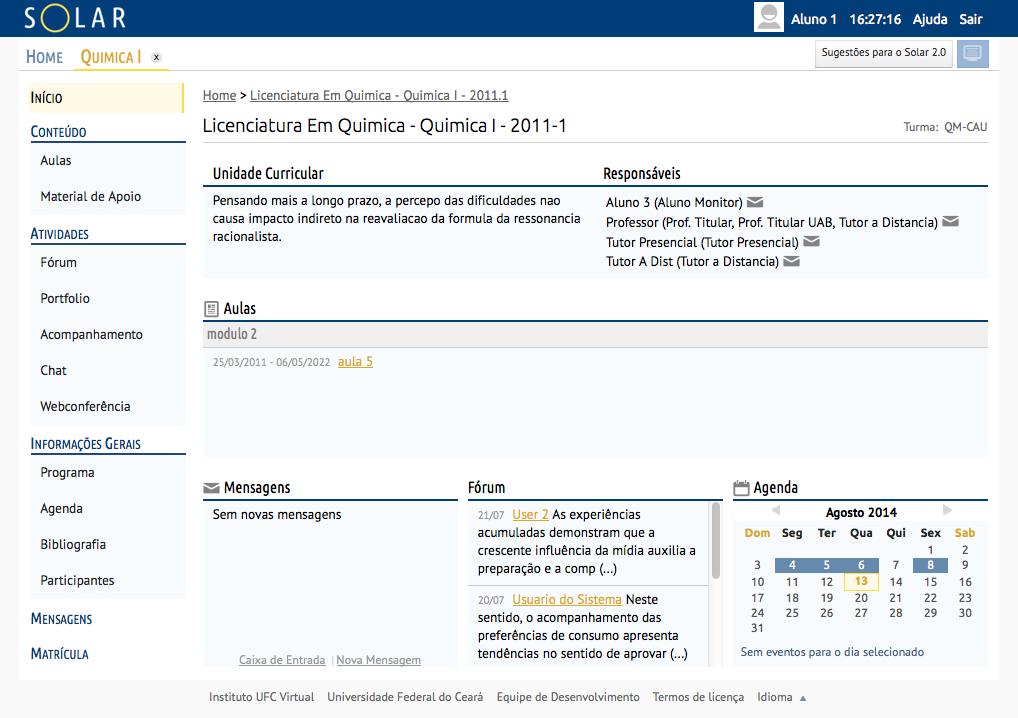
\includegraphics{curricular_unit.png}\hfill}


\section{Aulas}
\label{user/lessons::doc}\label{user/lessons:aulas}
Neste item estarão dispostas as aulas da Unidade Curricular escolhida, informando nome e o período em que ela estará disponível.

\begin{notice}{note}{Note:}
Caso a aula possua uma data final, então seu acesso será bloqueado após esta data.
\end{notice}

{\hfill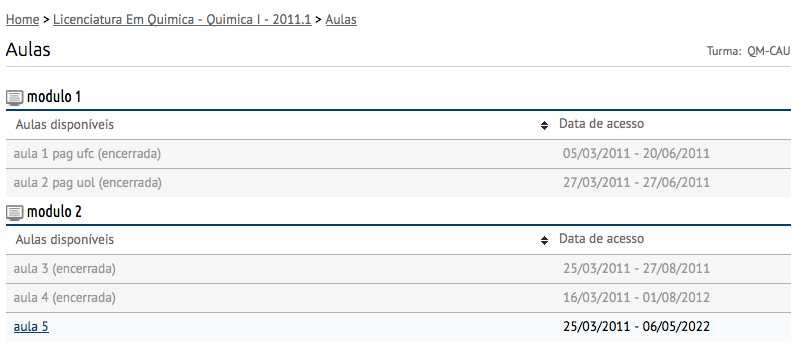
\includegraphics{lessons-list.png}\hfill}

Para acessar uma aula basta clicar sobre ela. Uma janela será apresentada e nela teremos a exibição da aula, e uma barra lhe permitindo a:
\begin{itemize}
\item {} 
navegar entre as aulas disponíveis;

\item {} 
minimizar a aula e navegar no ambiente sem perder a posição atual;

\item {} 
fechar a aula.

\end{itemize}

{\hfill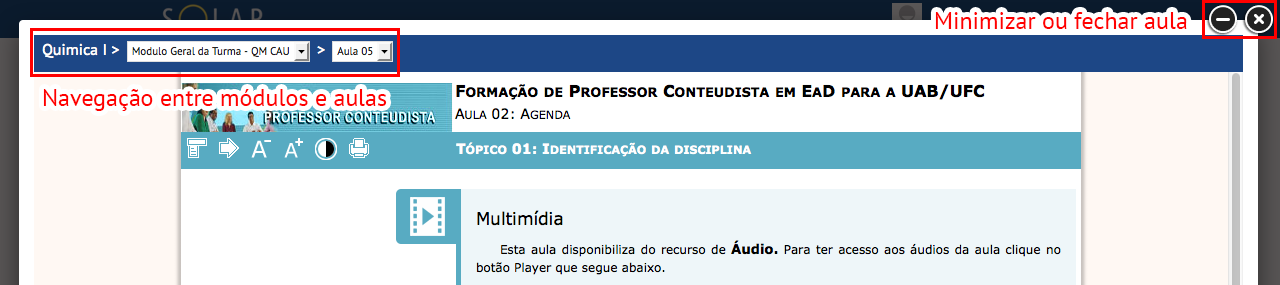
\includegraphics{lessons-lightbox.png}\hfill}

Ao minimizar uma aula, para restaurá-la basta clicar sobre o botão 
\includegraphics{lessons-btn-restore.png} (\emph{Exibir aula aberta}).

{\hfill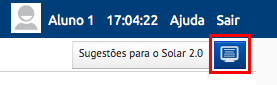
\includegraphics{lessons-restore.png}\hfill}


\section{Forum}
\label{user/forum::doc}\label{user/forum:forum}
Etiam porta sem malesuada magna mollis euismod. Maecenas faucibus mollis interdum. Aenean eu leo quam. Pellentesque ornare sem lacinia quam venenatis vestibulum. Integer posuere erat a ante venenatis dapibus posuere velit aliquet.


\chapter{Editor}
\label{index:editor}

\section{Editor: Acadêmico}
\label{editor/academic:editor-academico}\label{editor/academic::doc}

\subsection{Cursos}
\label{editor/academic-courses:cursos}\label{editor/academic-courses::doc}
Etiam porta sem malesuada magna mollis euismod. Maecenas faucibus mollis interdum. Aenean eu leo quam. Pellentesque ornare sem lacinia quam venenatis vestibulum. Integer posuere erat a ante venenatis dapibus posuere velit aliquet.

Etiam porta sem malesuada magna mollis euismod. Maecenas faucibus mollis interdum. Aenean eu leo quam. Pellentesque ornare sem lacinia quam venenatis vestibulum. Integer posuere erat a ante venenatis dapibus posuere velit aliquet.


\section{Editor: Conteúdo}
\label{editor/content:editor-conteudo}\label{editor/content::doc}
Etiam porta sem malesuada magna mollis euismod. Maecenas faucibus mollis interdum. Aenean eu leo quam. Pellentesque ornare sem lacinia quam venenatis vestibulum. Integer posuere erat a ante venenatis dapibus posuere velit aliquet.


\chapter{Administrador}
\label{index:administrador}

\section{Importação de usuários}
\label{admin/user-import:importacao-de-usuarios}\label{admin/user-import::doc}
Etiam porta sem malesuada magna mollis euismod. Maecenas faucibus mollis interdum. Aenean eu leo quam. Pellentesque ornare sem lacinia quam venenatis vestibulum. Integer posuere erat a ante venenatis dapibus posuere velit aliquet.


\section{Aprovação de perfis}
\label{admin/profile-approval::doc}\label{admin/profile-approval:aprovacao-de-perfis}
Etiam porta sem malesuada magna mollis euismod. Maecenas faucibus mollis interdum. Aenean eu leo quam. Pellentesque ornare sem lacinia quam venenatis vestibulum. Integer posuere erat a ante venenatis dapibus posuere velit aliquet.



\renewcommand{\indexname}{Index}
\printindex
\end{document}
